% !TeX spellcheck = it_IT
\documentclass[10pt,a4paper]{article}

\usepackage[utf8]{inputenc}
\usepackage[T1]{fontenc}	
\usepackage[italian]{babel}
\usepackage{amsmath}
\usepackage{amsfonts}
\usepackage{amssymb}
\usepackage{graphicx}

\usepackage[left=2cm,right=2cm,top=2cm,bottom=2cm]{geometry}
\geometry{a4paper}

\usepackage{booktabs} % for much better looking tables
\usepackage{verbatim}
\usepackage{subfig} % make it possible to include more than one captioned figure/table in a single 

\usepackage{fancyhdr} % This should be set AFTER setting up the page geometry
\pagestyle{fancy} % options: empty , plain , fancy
\renewcommand{\headrulewidth}{0pt} % customise the layout...
\lhead{}\chead{}\rhead{}
\lfoot{}\cfoot{\thepage}\rfoot{}

%%% SECTION TITLE APPEARANCE
\usepackage{sectsty}
%\allsectionsfont{\sffamily\mdseries\upshape} % (See the fntguide.pdf for font help)
% (This matches ConTeXt defaults)

% pacchetti che mi fanno schifo ma uso lo stesso (Bob è scemo, ma anche Ale...)
\usepackage[cdot, thickqspace, squaren]{SIunits}
% macro che mi piacciono
\def\code#1{\texttt{#1}}


\title{Esercitazione 6: Amplificatore operazionale\\ \Large{\emph{Circuiti lineari}}}

\author{Gruppo BE \\ Alessandro Candido, Roberto Ribatti}
\date{\today}
\begin{document}
\maketitle

\section{Scopo e strumentazione}
Misurare le caratteristiche di amplificatori invertenti e non invertenti realizzati con un op-amp TL081, da alimentare tra +15 V e -15V.
La strumentazione usata è quella presente sul banco di lavoro, più il suddetto transistor.

\section{Amplificatore invertente}

\subsection{$V_{out}$ in funzione di $V_{in}$}

\subsection{Impedenza d'ingresso}

\subsection{Risposta in frequenza}

\subsection{Slew rate}

\section{Amplificatore non invertente}

\section{Circuito integratore}

\subsection{Risposta in frequenza}
Si è misurata la risposta del circuito a un ingresso sinusoidale a varie frequenze. Si riportano i dati relativi in appendice in \tablename{\ref{tab:lowpass}}, e i grafici di seguito in \figurename{\ref{fig:lowamp}} e \figurename{\ref{fig:lowph}}.

\begin{figure}[h!]
	\centering
	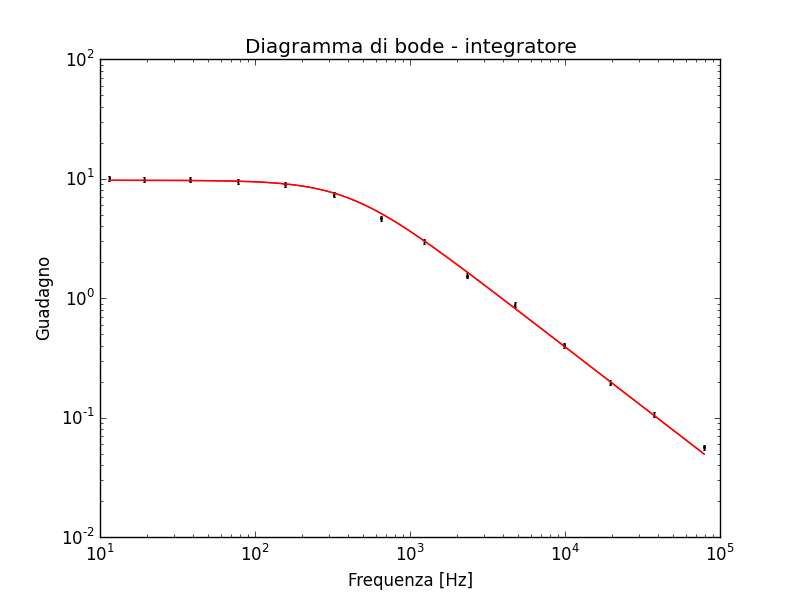
\includegraphics[width=0.65\textwidth]{../grafici/fit_module_low_pass.pdf}
	\caption{Grafico del fit }
	\label{fig:lowamp}
\end{figure}
\begin{figure}[h!]
	\centering
	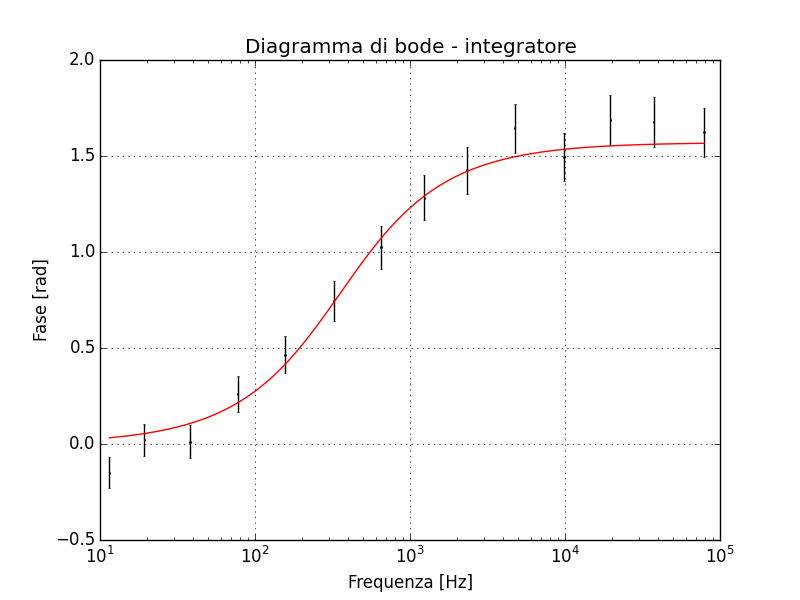
\includegraphics[width=0.65\textwidth]{../grafici/fit_phase_low_pass.pdf}
	\caption{Grafico del fit }
	\label{fig:lowph}
\end{figure}

Si riportano nella tabella di seguito i risultati del fit:

\begin{table}[h!]
\centering
\begin{tabular}{c|ccc}
amplitude	&	$A_0 = 11.20 \pm 0.27$	&	$f_0 = \unit{388 \pm 13}{\hertz}$	&	$\chi^2/ndof = 41.7 / 12$\\
phase		&	$\varphi_0 = \unit{-0.007 \pm 0.007}{\pi \rad}$	&	$f_0 = \unit{330 \pm 30}{\hertz}$	&	$\chi^2/ndof = 37.6 / 12$
\end{tabular}
\end{table}

\noindent Dove si sono usati i seguenti simboli:
\begin{itemize}
\item $A_0$ è il guadagno di centro banda, in questo caso è il guadagno a basse frequenze;
\item $\varphi_0$ è lo sfasamento per frequenze prossime allo 0;
\item $f_0$ è la frequenza di taglio dell'integratore.
\end{itemize}

% i chiquadri non sono splendidi e le due misure della frequenza di taglio poco compatibili, c'è da giustificare un minimo

\subsection{Risposta all'onda quadra}

% c'è da dire cosa ci si aspetta per l'ampiezza dell'onda in uscita, ci sono un sacco di armoniche...

Qualitativamente il comportamento osservato per la risposta del circuito all'onda quadra è esattamente quello di un integratore, almeno a $\unit{10}{\kilo\hertz}$, come si osserva dalla \figurename{\ref{fig:intsq}}.

\begin{figure}[h!]
	\begin{minipage}[t]{0.45\textwidth}
		\centering
		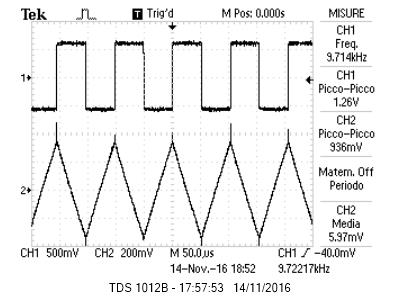
\includegraphics[width=1\textwidth]{../oscilloscopio/sqint.jpg}
	\end{minipage}
	\begin{minipage}[t]{0.45\textwidth}
		\centering
		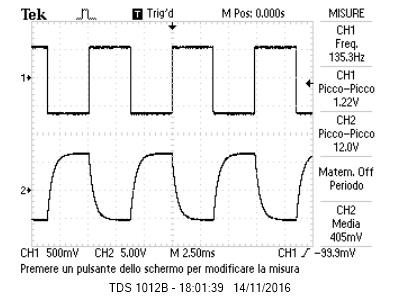
\includegraphics[width=1\textwidth]{../oscilloscopio/sqexp.jpg}
	\end{minipage}
	\caption{Risposta del circuito integratore a un'onda quadra in ingresso}
	\label{fig:intsq}
\end{figure}

Cambiando la frequenza del segnale di input si osserva che per frequenze maggiori il segnale viene ulteriormente attenuato, ma qualitativamente preserva il funzionamento come derivatore, mentre per frequenze più basse il condensatore ha il tempo di caricarsi e si può osservare una serie di esponenziali dovuti proprio a queste cariche e scariche, sempre in \figurename{\ref{fig:intsq}}.

\section{Circuito derivatore}

\subsection{Risposta in frequenza}

\subsection{Risposta all'onda triangolare}

\pagebreak
\section{Appendice: Dati}
Si riportano qui le tabelle di dati usati per i fit e i grafici.

\begin{figure}[h!]
	\centering
	\resizebox{0.7\textwidth}{!}{
	\input{../tabelle/tab_low_pass.txt}}
	\captionof{table}{Dati relativi al circuito integratore}
	\label{tab:lowpass}
\end{figure}

\begin{figure}[h!]
	\centering
	\resizebox{0.7\textwidth}{!}{
	\input{../tabelle/tab_high_pass.txt}}
	\captionof{table}{Dati relativi al circuito integratore}
	\label{tab:highpass}
\end{figure}

%\centering
%\begin{figure}[h!]
%	\begin{minipage}[t]{0.5\textwidth}
%		\centering
%		\resizebox{1\textwidth}{!}{
%		\input{../tabelle/tab_low_pass.txt}}
%		\captionof{table}{Dati relativi al circuito integratore}
%		\label{tab:lowpass}
%	\end{minipage}
%	\begin{minipage}[t]{0.5\textwidth}
%		\resizebox{1\textwidth}{!}{
%		\input{../tabelle/tab_high_pass.txt}}
%		\captionof{table}{Dati relativi al circuito integratore}
%		\label{tab:highpass}
%	\end{minipage}
%\end{figure}

\end{document}
